\documentclass[conference]{IEEEtran}
\IEEEoverridecommandlockouts
%Template version as of 04/05/2026

\usepackage{cite}
\usepackage{amsmath,amssymb,amsfonts}
\usepackage{graphicx}
\graphicspath{{./}{figures/}}
\usepackage{textcomp}
\usepackage{xcolor}
\usepackage{booktabs}
\usepackage{url}

%%%%%%%%%%%%% Needs to be added for header information
\usepackage{fancyhdr}
\setlength{\headheight}{24pt}
%%%%%%%%%%%%%%%%%%%%%%%%%%%%%%%%%%%%%

\def\BibTeX{{\rm B\kern-.05em{\sc i\kern-.025em b}\kern-.08em
    T\kern-.1667em\lower.7ex\hbox{E}\kern-.125emX}}

%%%%%%%%%%%%%% Needs to be added for header information
\fancypagestyle{firstpage}{%
 \fancyhf{}%
 \fancyhead[L]{10th International Artificial Intelligence and Data Processing Symposium (IDAP'26), Sept 5-6, 2026, Türkiye (Malatya – İstanbul), Philippines}
  
 \fancyfoot[L]{%%%% Copyright goes here
  \normalsize{979-8-3503-8359-1/24/\$31.00 ~\copyright2024 IEEE}
 }%
 \renewcommand{\headrulewidth}{0pt} % Remove the horizontal line in header
}
%%%%%%%%%%%%%%%%%%%%%%%%%%%%%%%%%%%%%

\begin{document}

\title{Optimized Related Work Generation with Multi Agent Systems}

\author{\IEEEauthorblockN{Hatice Nur K\"om\"urc\"u}
\IEEEauthorblockA{\textit{Department of Computer Engineering} \\
\textit{Izmir Institute of Technology}}
\and
\IEEEauthorblockN{Deniz Karabacak}
\IEEEauthorblockA{\textit{Department of Computer Engineering} \\
\textit{Izmir Institute of Technology}}
\and
\IEEEauthorblockN{Emrah İnan}
\IEEEauthorblockA{\textit{Department of Computer Engineering} \\
\textit{Izmir Institute of Technology}}
}

\maketitle

%%%%%%%%%%%%%%%% Needs to be added for header information
\thispagestyle{firstpage}
%%%%%%%%%%%%%%%%%%%%%%%%%%%%%%%%%%%%%

\begin{abstract}
Writing the Related Work section of an academic paper requires reasoning information from multiple documents while identifying gaps in the literature. While authors often miss recent papers in a time consuming process, single agent LLM models often produce shallow, sequential summaries and may hallucinate citations. We present a local, autonomous Multi Agent System (MAS) that decomposes related work generation into planning, outlining, parallelized writing, and a critic driven revision loop. We benchmark our MAS against a single agent baseline on a high reference subset of OARelatedWork and report lexical, semantic, citation quality, and LLM judge (GRC) metrics. On 10 high reference samples (minimum 7 references), the MAS substantially improves grounding and citation precision, at the cost of higher runtime.
\end{abstract}

\begin{IEEEkeywords}
related work generation, multi agent systems, large language models, citation quality, automated research writing
\end{IEEEkeywords}

\section{Introduction}
Writing a Related Work section is among the most demanding parts of research writing. Authors must retrieve relevant publications, compare methods and findings, organize papers into coherent themes, and explain how their contribution differs from prior work all while maintaining accurate citations and an appropriate academic tone. As literature volume grows, this process becomes increasingly slow and error prone: important papers may be missed, summaries can collapse into sequential abstracts, and unsupported claims may slip into the final text.

Automating related work generation has therefore attracted interest as a hard NLP task rather than a generic summarization problem. Early and recent systems treat it as target aware synthesis: the model must write prose that is grounded in a provided reference set, aligned with the target paper, and structured as a review rather than a list of paper descriptions \cite{chen2022tag,scireviewgen2023,surge2025}. Datasets such as SciReviewGen and OARelatedWork provide ground truth related work sections and reference lists for evaluation, while benchmark frameworks such as SURGE stress multidimensional assessment beyond lexical overlap \cite{surge2025,scireviewgen2023}. Together with expert and automatic evaluations \cite{expertEvalRW2025,sahinuc2024citationtext}, this line of work shows that a strong related work section must group papers into themes, cite sources correctly, and explain what prior work has not yet solved. High word overlap with reference text, as measured by ROUGE, is not enough on its own.

Large language models (LLMs) make this automation plausible. Their strong language understanding and generation capabilities support abstractive synthesis across many source abstracts in a single pass. Yet LLM outputs for research writing remain unreliable: models may hallucinate citations, paraphrase sources without faithful grounding, or produce fluent but shallow text that reads like a combination of summaries rather than a comparative review \cite{expertEvalRW2025,li2024ceg}. These failures are especially critical in related work, where every claim is expected to trace back to cited evidence.

The recent development has been the single agent pipeline: one LLM instance retrieves context, plans themes, drafts the section, and optionally self critiques in a single workflow. This design is simple and fast, but it concentrates planning, synthesis, and verification in one long prompt. Under many references and long contexts, the model tends toward sequential listing, weak transitions, little comparison with prior work, and inconsistent citation usage. Post verification methods such as Citation Enhanced Generation (CEG) improve grounding after generation \cite{li2024ceg}, but they do not address the structural bottleneck of single agent writing.

Multi agent systems (MAS) offer a complementary design: specialized agents handle planning, outlining, writing, and quality control separately, with explicit communication and revision loops \cite{lira2025,agentLaboratory2025,li2024masSurvey}. For related work generation, such decomposition allows thematic planning and citation assignment before drafting, parallel section writing, and a critic that rejects ungrounded drafts before assembly. In this paper, we present a local MAS with Planner, Outliner, parallel Writers, and Critic agents, served on Qwen3-8B via vLLM. We benchmark it against a single agent baseline on a high reference subset of the OARelatedWork dataset.

Our contributions are: (i) a local MAS for related work generation with planning, outlining, parallel writing, and critic based revision; (ii) citation pre assignment coupled with a strict critic loop to improve factual grounding; (iii) multidimensional evaluation on a high reference subset of OARelatedWork (lexical, semantic, citation, and GRC metrics); and (iv) qualitative and quantitative analysis of how MAS trades reference overlap for improved grounding and citation coverage.

\section{Related Work}
\label{sec:related_work}
Literature review and survey generation have recently gained attention as a distinct evaluation target, including benchmark construction and standardized evaluation protocols.
SURGE proposes a benchmark and evaluation framework for scientific survey generation, emphasizing multidimensional evaluation beyond lexical overlap \cite{surge2025}.
SciReviewGen is a large scale dataset for automatic literature review generation and has been used in subsequent systems and evaluations \cite{scireviewgen2023}.
FutureGen uses a retrieval augmented generation (RAG) pipeline to draft future work sections from a target paper and retrieved literature, illustrating retrieval conditioned scholarly writing as a complementary task to related work synthesis \cite{azher2025futuregen}.

Recent work also highlights that automatic metrics alone are insufficient for scholarly writing quality.
Expert preference based evaluation frameworks for related work generation provide human aligned assessment dimensions such as coherence and scholarly appropriateness \cite{expertEvalRW2025}.
\c{S}ahinu\c{c} et al.~\cite{sahinuc2024citationtext} systematically explore citation text generation with LLMs and show that prompt design and input configuration strongly affect outputs, while lexical, semantic, and human judgment metrics can diverge. This motivates our multi metric protocol on OARelatedWork (ROUGE/BERTScore, citation precision/recall/F1, and GRC judge scores).

More directly, Chen et al.~\cite{chen2022tag} study related work generation as a target aware abstractive task and use contrastive learning to better align generated related work with the target paper and cited literature.
Liu et al.~\cite{liu2025selectreadwrite} propose a multi agent framework for full text based related work generation that separates selection, reading, and writing.
In contrast, this work presents a local MAS with an explicit critic loop and evaluates citation quality (precision/recall/F1) and grounding alongside ROUGE/BERTScore/LSA.

Citation grounding remains a critical bottleneck in scholarly generation.
Li et al.~\cite{li2024ceg} propose Citation Enhanced Generation (CEG), a training free post hoc framework that retrieves supporting evidence and applies natural language inference to verify claims, regenerating responses until statements are citation backed.
Our critic driven revision loop pursues the same goal during generation. The outliner pre assigns citation keys, the critic rejects ungrounded drafts, and verification runs section wise within a multi agent pipeline.

On the systems side, multi agent approaches (e.g., LiRA) decompose review writing into specialized roles and incorporate reliability mechanisms to improve readability and reduce hallucinations \cite{lira2025}.
General agent development environments (e.g., Agent Laboratory) motivate modular agent roles and iterative research workflows for LLM agents \cite{agentLaboratory2025}.
Li et al.~\cite{li2024masSurvey} survey LLM based multi agent systems across workflow patterns, infrastructure, and challenges such as coordination, memory, and hallucination control; our planner, outliner, writer, and critic design instantiates such role decomposition for the related work generation task.

\section{Method}
\label{sec:method}

\subsection{Single Agent}
We implement an end to end pipeline for the single agent model in which one LLM instance performs retrieval context reading, planning, logical reasoning, and gap analysis in a single generation step, with optional self critique refinement. In both the Single Agent and MAS, the input consists of (i) a target paper descriptor (title/topic, optionally an abstract and fields of study) and (ii) a set of candidate papers (typically abstracts) that the system should cite and synthesize.

In interactive mode, the retrieval process uses the arXiv API: given a user query, the agent requests the top-5 most relevant papers and constructs a compact per paper context containing title, authors, year, and abstract. Each paper is also assigned an author year citation string (e.g., \texttt{(Smith et al., 2020)}) derived from the first author's surname and publication year to encourage consistent citations in generation. In benchmark mode, retrieval is disabled, and the agent is directly provided with the paper contexts from OARelatedWork.

The generation step concatenates the paper contexts into a single prompt and asks the model to produce 2--4 paragraphs of continuous prose with thematic grouping, smooth transitions, and an explicit gap analysis at the end. Prompts explicitly require that every factual claim be grounded with an author year citation. If enabled, a second pass performs self critique and rewrites the draft to fix missing citations, weak transitions, and missing gap analysis. Implementation wise, this pipeline is represented as a small LangGraph with the nodes \texttt{retrieve} $\rightarrow$ \texttt{generate} $\rightarrow$ \texttt{critique} $\rightarrow$ \texttt{finalize}. This model is simple and fast, but a single prompt must jointly solve planning, synthesis, and fact checking; under long context pressure it can degrade into sequential paper listing, shallow synthesis, and citation errors. This motivated the parallel MAS design.

This motivated the parallel MAS design.

\begin{figure}[t]
  \centering
  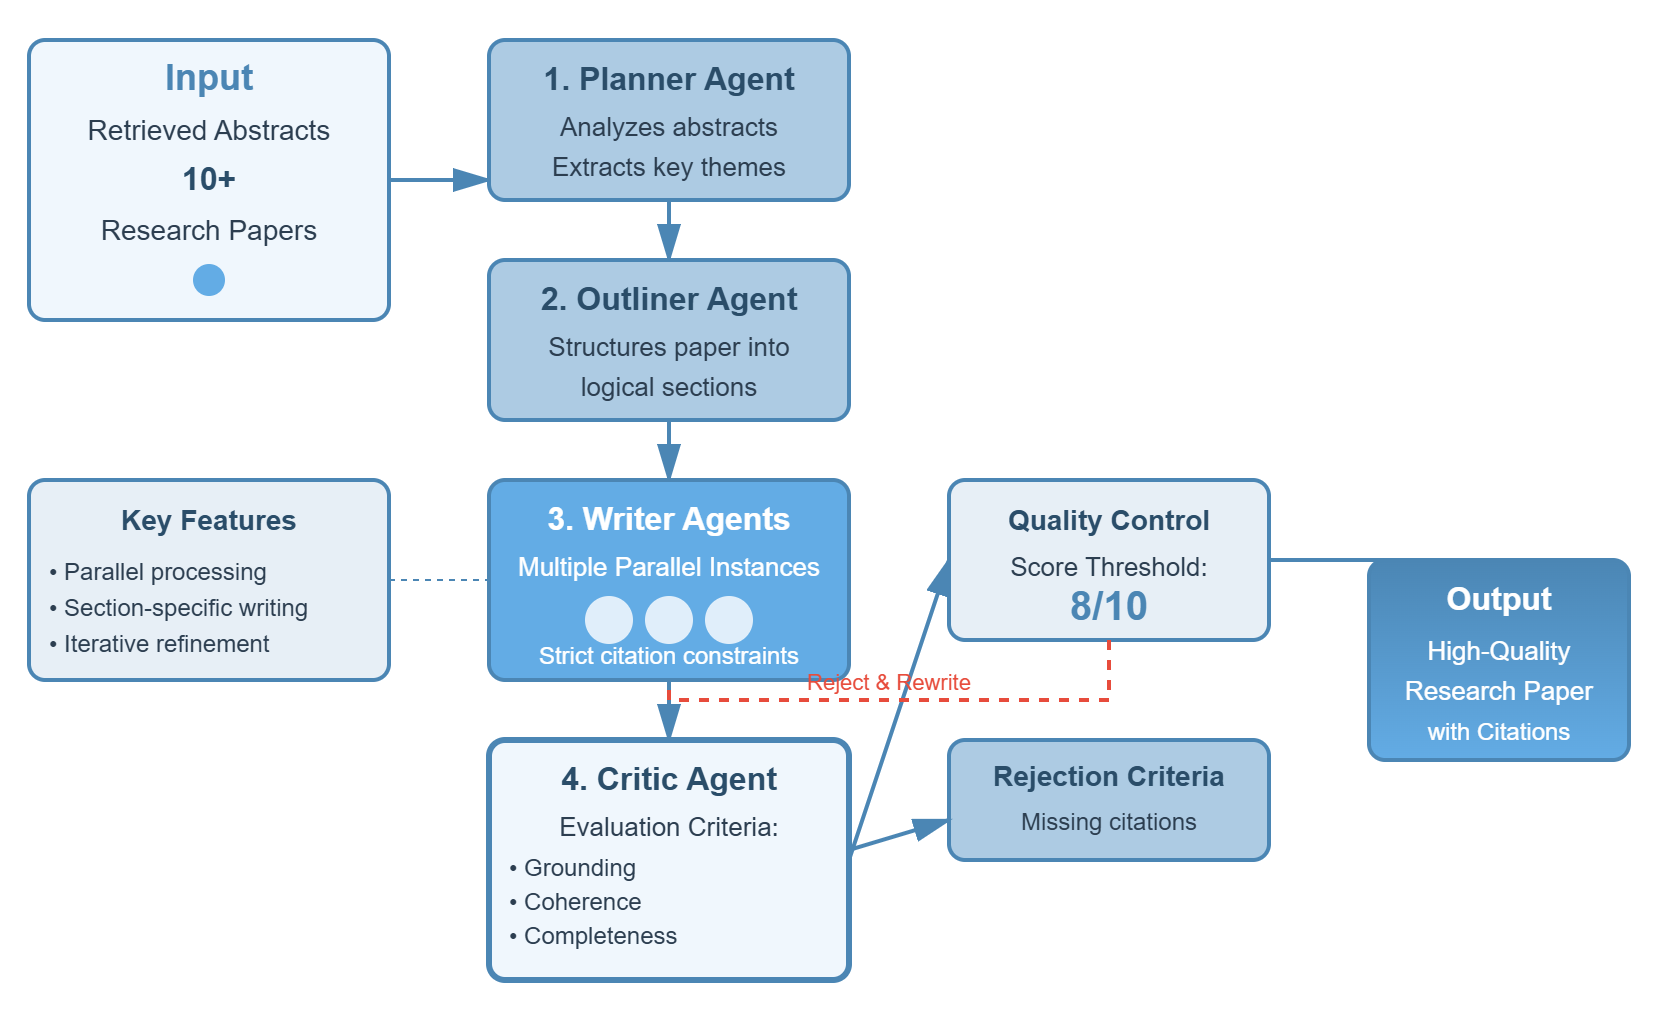
\includegraphics[width=\linewidth]{multi_agent_workflow.png}
  \caption{Multi agent workflow (Planner $\rightarrow$ Outliner $\rightarrow$ parallel Writers $\leftrightarrow$ Critic $\rightarrow$ assembly).}
  \label{fig:workflow}
\end{figure}

\subsection{Multi Agent System}
Our multi agent system decomposes the same input into four specialized roles so that planning, writing, and quality control are handled separately (Fig.~\ref{fig:workflow}). All agents call the same locally hosted Qwen3-8B model (4-bit quantized) through vLLM's OpenAI compatible API \cite{vllm2023,qwen3}. vLLM batches concurrent requests efficiently, which makes parallel section generation practical on one GPU. LangGraph orchestrates the pipeline \cite{langgraph}.

The Planner reads all candidate paper abstracts and groups them into two to four themes. It clusters related papers under each theme so later stages write about coherent topics rather than isolated summaries. Its output is passed directly to the Outliner.

The Outliner turns each theme cluster into a section plan. For every section, it assigns the papers to cite and fixes citation keys before any text is generated. This pre assignment step is the main structural difference from the single agent baseline: citations are decided during planning, not added afterward.

Each section is then handled by a Writer agent. The Writer receives the section plan, the assigned papers, and a length budget based on how many citations the section must cover. It produces one paragraph of continuous academic prose and must use all assigned citation keys. Multiple Writers run in parallel through a thread pool with up to three workers. Each worker sends one section prompt to vLLM, receives the draft, and immediately passes it to the Critic. Rejected sections are revised in later rounds without blocking other sections. Writers use Qwen3 thinking mode (top-$p=0.95$); the Critic uses a lower temperature (0.2) for stable scoring.

The Critic evaluates each section draft before assembly. It scores Grounding (whether claims are supported by assigned sources), Coherence (logical flow within the section), and Completeness (coverage of assigned papers and themes). It also checks citation accuracy as the fraction of pre assigned keys present in the text. A section is accepted only when all three GRC scores reach 9 and citation accuracy meets the minimum threshold. If a section fails, the Critic returns feedback and the same Writer revises it. Each section may be revised up to two times; sections that still fail are force assembled so the pipeline can finish. Accepted sections are combined into the final related work text and condensed if the output exceeds the reference length.

In benchmark mode, retrieval is disabled and the system consumes paper contexts from OARelatedWork. In interactive mode, papers are retrieved from the arXiv API before the Planner runs.

\section{Evaluation}
\label{sec:evaluation}

\subsection{Dataset and Protocol}
We evaluate on OARelatedWork, which provides (i) a ground truth Related Work section and (ii) its reference list. We filter to samples with at least 7 references and take the first 10 qualifying samples in streaming order. The selected samples average 11.6 references each. Both systems use Qwen3-8B (4-bit) served through vLLM with top-$p=0.95$ sampling. Role temperatures are 0.4 for Planner and Outliner, 0.7 for Writer, and 0.2 for Critic. The MAS allows up to 2 revision rounds per section and accepts a section only when all GRC scores reach 9. LSA is computed in a TF IDF space enriched with source paper context. All GRC scores use an LLM based judge without human evaluation. Code and JSON traces are available at \url{https://github.com/Denizdius/mas_project}.

\subsection{Metrics}
We report lexical overlap (ROUGE-1/2/L, METEOR, chrF), semantic similarity (BERTScore and LSA similarity), citation quality (precision, recall, F1, and citation density), LLM judge quality (GRC: Grounding, Coherence, Completeness), and efficiency (runtime per sample). Win rate counts the fraction of samples where MAS exceeds the single agent baseline on a given metric (ties reported separately). MAS success rate is the fraction of samples where every section was accepted by the critic at least once during revision.

\subsection{Aggregate Results}
Table~\ref{tab:results} summarizes average scores on the shared evaluation set. Lexical overlap is nearly unchanged: ROUGE-1, ROUGE-2, and ROUGE-L differ by less than 0.01 between systems, and BERTScore stays close (0.840 vs.\ 0.836). The clearest lexical shift is LSA similarity, which drops from 0.622 for the single agent to 0.401 for MAS. This indicates that MAS writes more abstractive text that overlaps less with the reference wording.

Citation quality improves substantially under MAS. Precision rises from 0.796 to 0.960, recall from 0.721 to 1.690, and F1 from 0.735 to 1.214. The recall value above 1.0 reflects denser citation usage in generated text rather than perfect reference matching. GRC Grounding increases from 4.7 to 8.15, the largest quality gain in the benchmark. Completeness also improves (6.1 to 7.32), while Coherence remains high for both systems (9.2 vs.\ 8.92). These results show that role decomposition and critic based revision improve factual support and citation coverage more than surface overlap.

The main cost is runtime: MAS needs 318.8 seconds per sample compared with 67.0 seconds for the single agent (${\sim}$4.8$\times$ slower). This overhead comes from multiple agent calls, parallel section writing, and up to two critic driven revision rounds per section. For applications where grounding matters more than latency, the quality gains justify the extra compute.

\begin{table}[t]
\caption{Benchmark results on OARelatedWork high reference subset ($n=10$, min refs=7). Higher is better except runtime.}
\label{tab:results}
\centering
\small
\begin{tabular}{lcc}
\toprule
\textbf{Metric} & \textbf{Single Agent} & \textbf{MAS} \\
\midrule
ROUGE-1 & 0.392 & 0.383 \\
ROUGE-2 & 0.099 & 0.099 \\
ROUGE-L & 0.159 & 0.158 \\
BERTScore & 0.840 & 0.836 \\
LSA similarity & 0.622 & 0.401 \\
\midrule
Citation precision & 0.796 & 0.960 \\
Citation recall & 0.721 & 1.690 \\
Citation F1 & 0.735 & 1.214 \\
\midrule
GRC Grounding & 4.7 & 8.15 \\
GRC Coherence & 9.2 & 8.92 \\
GRC Completeness & 6.1 & 7.32 \\
\midrule
Time/sample (s) & 67.0 & 318.8 \\
\bottomrule
\end{tabular}
\end{table}
\vspace{0.6\baselineskip}

Table~\ref{tab:extended} reports additional statistics. Higher MAS citation density (5.42 vs.\ 2.41 cites per 100 words) explains recall above 1.0; higher abstractiveness (1.00 vs.\ 0.98) and length control (ratio 1.00 vs.\ 1.10) align with the lower LSA in Table~\ref{tab:results}.

\begin{table}[t]
\caption{Extended lexical and citation statistics (means over $n=10$).}
\label{tab:extended}
\centering
\small
\begin{tabular}{lcc}
\toprule
\textbf{Metric} & \textbf{Single Agent} & \textbf{MAS} \\
\midrule
METEOR & 0.245 & 0.240 \\
chrF & 0.424 & 0.445 \\
Citation density (generated) & 2.41 & 5.42 \\
Length ratio & 1.10 & 1.00 \\
Abstractiveness & 0.981 & 1.000 \\
\bottomrule
\end{tabular}
\end{table}

\subsection{Per Sample Analysis}
Table~\ref{tab:winrate} formalizes paired comparisons across the 10 benchmark samples. MAS wins on Grounding in 10/10 cases and on Completeness in 8/10, but Coherence is split (2 wins, 4 ties, 4 losses). The overall win rate (8/10) counts samples where MAS wins on at least 3 of 5 core metrics. Across all samples, the MAS executed 57 critic writer revision cycles ($\sim$5.7 per sample); only 3/10 achieved full critic acceptance on every section, with remaining sections force assembled after 2 revision rounds. The MAS is ${\sim}$4.8$\times$ slower but improves accuracy related metrics when grounding matters more than raw latency.

\begin{table}[t]
\caption{Per metric win rates on the 10 sample paired benchmark.}
\label{tab:winrate}
\centering
\small
\begin{tabular}{lccc}
\toprule
\textbf{Metric} & \textbf{MAS Wins} & \textbf{Ties} & \textbf{Losses} \\
\midrule
GRC Grounding & 10 & 0 & 0 \\
GRC Coherence & 2 & 4 & 4 \\
GRC Completeness & 8 & 1 & 1 \\
Citation Recall & 9 & 1 & 0 \\
Citation Precision & 5 & 1 & 4 \\
\midrule
Overall ($\geq$3 of 5) & \multicolumn{3}{c}{8/10 samples} \\
\bottomrule
\end{tabular}
\end{table}

\subsection{Qualitative Output Comparison}
To complement automatic metrics, we inspect paired outputs on one high reference word senses example (19 references), where the single agent reaches LSA 0.946 (GRC Grounding 5) and MAS reaches LSA 0.659 (GRC Grounding 9.3). The single agent output closely follows the reference phrasing:
\begin{quote}\small
Recent years have seen a surge in semantic representation research, largely driven by word embeddings like Word2Vec (Mikolov et al., 2013) and GloVe (Pennington et al., 2014)\ldots\ Li and Jurafsky (2015) introduced a multi-sense embedding pipeline\ldots\ Flekova and Gurevych (2016) developed supersense embeddings for classification tasks.
\end{quote}
The MAS output is organized into thematic sections with denser citation coverage:
\begin{quote}\small
The study of polysemy in natural language processing has driven extensive research into modeling sense-specific representations\ldots\ Pilehvar et al. (2016) introduced de-conflated semantic representations\ldots\ Suster et al. (2016) extended this with bilingual multi-sense embeddings\ldots\ Camacho-Collados et al. (2016) integrated explicit knowledge with corpus statistics in Nasari\ldots
\end{quote}
This illustrates the grounding and overlap trade off: MAS produces more abstractive, citation rich synthesis at the cost of lexical similarity to the reference. Full generated texts for this example are provided in the Appendix.

\section{Conclusion}
\label{sec:conclusion}
We presented a local Multi Agent System for automated related work generation that decomposes the task into planning, outlining, parallel writing, and critic based revision.
On a high reference subset of OARelatedWork ($n=10$), the MAS improves factual grounding and citation precision compared to a single agent baseline, at the cost of higher runtime.

Promising directions include: (i) calibrating the critic with human feedback, (ii) improving citation matching to avoid recall values above 1.0, (iii) integrating an explicit citation graph to support theme discovery and gap analysis, and (iv) scaling to larger and more diverse benchmarks \cite{scireviewgen2023,surge2025}.

\bibliographystyle{IEEEtran}
\bibliography{references}

\section*{Appendix: Full Generated Outputs}
\subsection*{Single Agent Output}
\small
Recent years have seen a surge in semantic representation research, largely driven by word embeddings like Word2Vec (Mikolov et al., 2013) and GloVe (Pennington et al., 2014). These embeddings were quickly adopted in NLP due to the rise of deep learning. This trend extended to sense representation, with techniques proposed to cluster contexts (Sch\"utze, 1998; Reisinger and Mooney, 2010; Huang et al., 2012) or use external inventories. Despite this, integrating sense representations remains challenging. Li and Jurafsky (2015) introduced a multi-sense embedding pipeline to test their utility. Flekova and Gurevych (2016) developed supersense embeddings for classification tasks.

\subsection*{MAS Output}
\small
The study of polysemy in natural language processing has driven extensive research into modeling sense-specific representations, with early work focusing on disentangling word senses from general embeddings. Pilehvar et al. (2016) introduced de-conflated semantic representations, separating word senses from general embeddings to address polysemy through sense-specific vectors. Suster et al. (2016) extended this with bilingual multi-sense embeddings, using discrete autoencoders and parallel corpora to align sense representations across languages. Flekova and Gurevych (2016) proposed supersense embeddings, enabling simultaneous sense classification and utilization via unified models. Mancini et al. (2016) combined lexical knowledge and distributional statistics in joint training to refine sense-specific embeddings. Li and Jurafsky (2015) demonstrated that multi-sense embeddings improve tasks like sentiment analysis by capturing sense-specific semantics. Ettinger et al. (2016) retrofitted sense-specific vectors using parallel text, aligning embeddings with linguistic constraints. Rothe et al. (2015) extended word embeddings to synsets via AutoExtend, mapping lexical units to semantic primitives. Iacobacci et al. (2015) developed SensEmbed to model sense-level similarity, enhancing disambiguation through relational embeddings. Guo et al. (2014) pioneered sense-specific embeddings using bilingual resources, leveraging cross-linguistic parallels. Camacho-Collados et al. (2016) integrated explicit knowledge with corpus statistics in Nasari, creating multilingual concept representations. These studies collectively highlight diverse strategies for scalable, context-aware modeling, emphasizing the interplay between explicit knowledge (Camacho-Collados et al., 2016) and autoencoder-based methods (Suster et al., 2016) in addressing sense disambiguation.

Sch\"utze (1998) pioneered automated word sense discrimination by leveraging distributional patterns to identify distinct meanings of polysemous words, laying the groundwork for sense-level representation. Reisinger et al. (2010) extended this by introducing multi-prototype vector-space models, explicitly representing multiple senses as distinct vectors to enable fine-grained differentiation. Huang et al. (2012) further refined this approach by incorporating global context and multiple word prototypes, enhancing the ability to capture nuanced semantic relationships. Concurrently, Mikolov et al. (2013) and Pennington et al. (2014) developed scalable word embedding methods, Word2Vec and GloVe, respectively, which encode words as dense vectors based on co-occurrence statistics. While these models excel at capturing general semantic similarity, they lack explicit mechanisms for disambiguating senses. Tian et al. (2014) addressed this by proposing a probabilistic framework for learning multi-prototype embeddings, allowing words to associate with multiple latent semantic prototypes, thereby aligning with Reisinger's multi-prototype approach.

\end{document}
